\documentclass{exam}

\ProvidesPackage{preamble}
\usepackage{amsmath}
\usepackage{graphicx}
\usepackage{physics}

\usepackage{pgfplots}
    \pgfplotsset{width=7cm,compat=1.18}
\usepackage{hyperref}
\usepackage{tikz} %tikz is used to draw the glyphs
\usepackage{tikz-3dplot}
\usepackage{mathtools}
\usetikzlibrary{arrows.meta, bending}
\usetikzlibrary{shapes.geometric}
\makeatletter

\pagestyle{head}
\firstpageheader{PHYS.4340L\\Quantum Information Lab}{UMASS-Lowell\\}{Matthew Jarek\\\today}
\runningheader{PHYS.4340L\\}{UMASS-Lowell\\}{M. Jarek\\\thepage}

\qformat{\textbf{Problem \questionlabel}\hfill}
%\qformat{\textbf{Question \thequestion}\hfill}

\renewcommand{\solutiontitle}{\noindent\textbf{Solution:}\par\noindent}
\newcommand{\st}[0]{$^\text{st}$ }
\newcommand{\nd}[0]{$^\text{nd}$ }
\renewcommand{\abs}[1]{\left|{#1}\right|}
\newcommand{\p}[1]{{\left({#1}\right)}}
\newcommand{\ds}{\displaystyle}
\renewcommand{\k}{\frac{1}{4\pi\epsilon_0}}
\renewcommand{\outer}[2]{\ket{#1}\bra{#2}}
\newcommand{\inner}[2]{\bra{#1}\ket{#2}}

\begin{document}
\begin{center}
    \Large
\textbf{Lab 5: Quantum Computing Workshop}
\end{center}
    \section{Superpostion}
    \subsection{Calculations}
    We start with defining a basis state of $\ket{0}$:
    \begin{equation*}
        \ket{0} = \begin{pmatrix}
            1\\0
        \end{pmatrix}.
    \end{equation*}
    To put the state in superpostion, the Hadamard gate needs to be applied.
    \begin{equation}
        \ket{0} = 
        \begin{pmatrix}
            1\\0
        \end{pmatrix}
        \xrightarrow{Hadamard} H\ket{0} = 
        \frac{1}{\sqrt{2}}
        \begin{pmatrix}
        1 & 1\\ 1 & -1    
        \end{pmatrix}
        \begin{pmatrix}
            1\\0
        \end{pmatrix} = 
        \frac{1}{\sqrt{2}}\left[\begin{pmatrix}
            1\\0
        \end{pmatrix} + \begin{pmatrix}
            0\\1
        \end{pmatrix}\right] = \ket{+}
    \end{equation}
    Comparting this to the general form of a qubit state in the given basis (where $\ket{1} = (^0_1)$):
    \begin{equation}
        \ket{\psi} = \alpha \ket{0} + \beta \ket{1},
    \end{equation}
    we can say that $\alpha = \beta = \frac{1}{\sqrt{2}}$ which means that ${\left|\alpha\right|}^2 = {\left|\beta\right|}^2 = {\left|\frac{1}{\sqrt{2}}\right|}^2 = .5$, or there is a 50/50 chance of being in ether state.
    \subsection{Code}
    The circuit needed to implement the superpostion is shown below.
    \begin{center}
            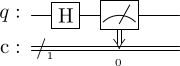
\includegraphics[width = .17 \linewidth]{images/Lab5_part1_circuit.png}
    \end{center}
    For reproducability the code that was used to simulate the quantum circuit is provided.
    \begin{verbatim}
        qc_super = QuantumCircuit(1,1)
        qc_super.h(0)
        qc_super.measure(0,0)
        shots_super = 1024
        job_super = simulator.run([qc_super], shots = shots_super)
        plot_histogram(job_super.result().get_counts(0))
    \end{verbatim}
    \subsection{Results}
    \begin{center}
        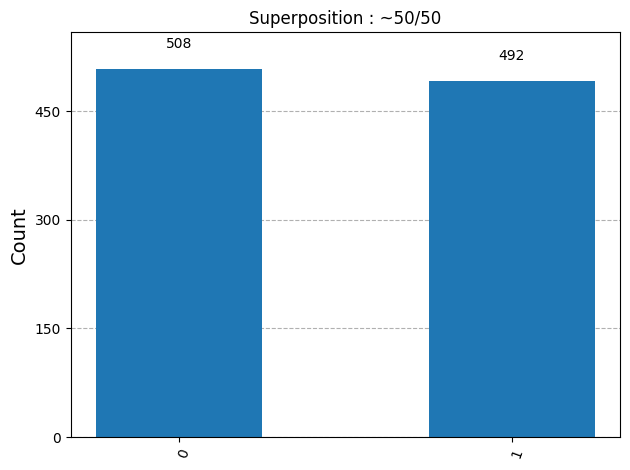
\includegraphics[width = .7 \linewidth]{images/Lab5_part1_hist.png}
    \end{center}
    The result of the simulation shows that the number of shots that were measured in the $\ket{0}$ state was 508 compared to the 492 shots measured in $\ket{1}$.
    The total number of shots ran was 1000, which means we had $\frac{508}{1000} \approx 51\%$ of the measurements result in $\ket{0}$ and $\frac{492}{1000} \approx 49\%$ of the measurements result in $\ket{1}$ which is within the 5\% error margin expected.
    \section{Bell State}
    \subsection{Calculations}
    We now have two qubits which means a new set of basis states are defined.
    \begin{equation*}
        \ket{00} = \begin{pmatrix} 1\\0\\0\\0 \end{pmatrix}, \quad
        \ket{01} = \begin{pmatrix} 0\\1\\0\\0 \end{pmatrix}, \quad
        \ket{10} = \begin{pmatrix} 0\\0\\1\\0 \end{pmatrix}, \quad
        \ket{11} = \begin{pmatrix} 0\\0\\0\\1 \end{pmatrix}. 
    \end{equation*}
    By starting with an initial state of $\ket{00}$ we can apply $H \otimes I$ then CNOT to create a Bell State.
    \begin{equation}
        \left(H \otimes I\right)\ket{00} = 
        H\ket{0} \otimes I\ket{0} = 
        \ket{+} \otimes \ket{0} = 
        \frac{1}{\sqrt{2}}\left(\ket{00} + \ket{10}\right),
    \end{equation}
    where the result of Eq. 1 was used to calculate $H\ket{0}$ and the main property of the Identity matrix was used to calculate $I\ket{0}$.
    \begin{equation}
        \text{CNOT}\left(H \otimes I\right)\ket{00} = 
        \text{CNOT}\frac{1}{\sqrt{2}}\left(\ket{00} + \ket{10}\right) =
        \frac{1}{\sqrt{2}}\left(\ket{0}\!\!\bra{0} \otimes I + \ket{1}\!\!\bra{1} \otimes X\right)\left(\ket{00} + \ket{10}\right) = \frac{1}{\sqrt{2}}\left(\ket{00} + \ket{11}\right)
    \end{equation} 
    This result is similar to Part 1, but now we should have a 50/50 chance of our result being in $\ket{00}$ or $\ket{11}$ instead of $\ket{0}$ or $\ket{1}$.
    \subsection{Code}
    The circuit to implement the bell states is shown below.
    \begin{center}
            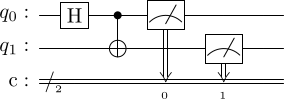
\includegraphics[width = .27 \linewidth]{images/Lab5_part2_circuit.png}
    \end{center}
    For reproducability the code that was used to simulate the quantum circuit is provided.
    \begin{verbatim}
        qc_bell = QuantumCircuit(2,2)
        qc_bell.h(0)
        qc_bell.cx(0,1)
        qc_bell.measure(0,0)
        qc_bell.measure(1,1)
        shots_bell = 1024
        job_bell = simulator.run([qc_bell], shots = shots_bell)
        plot_histogram(job_bell.result().get_counts(0))
    \end{verbatim}
    \subsection{Results}
    \begin{center}
        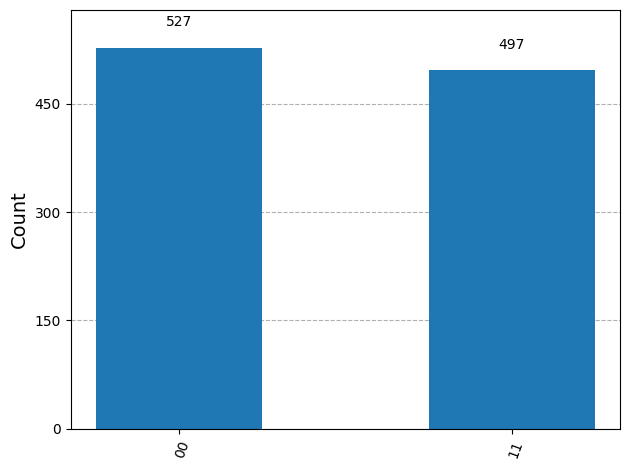
\includegraphics[width = .7 \linewidth]{images/Lab5_part2_hist.png}
    \end{center}
    The result of the simulation shows that the number of shots that were measured in the $\ket{00}$ state was 527 compared to the 497 shots measured in $\ket{11}$.
    The total number of shots ran was 1024, which means we had $\frac{527}{1024} \approx 51\%$ of the measurements result in $\ket{00}$ and $\frac{497}{1024} \approx 49\%$ of the measurements result in $\ket{11}$ which is within the 5\% error margin expected.
    These percentages add up to 100\%, which is expected as the only two results shown in the histogram are $\ket{00}$ and $\ket{11}$.
    \section{Modified Bell}
    \subsection{Calculations}
    Using the same basis states and circuit from part 2, we modify the circuit and add a X (bit-flip) gate to qubit 1 (the second qubit) before the CNOT.
    This means we are now starting with an initial state of $\ket{00} \xrightarrow{I \otimes X} \ket{01}$, then apply $H \otimes I$ then CNOT to create a Modified Bell State.
    \begin{equation}
        \left(H \otimes I\right)\ket{01} = 
        H\ket{0} \otimes I\ket{1} = 
        \ket{+} \otimes \ket{1} = 
        \frac{1}{\sqrt{2}}\left(\ket{01} + \ket{11}\right),
    \end{equation}
    where the result of Eq. 1 was used to calculate $H\ket{0}$ and the main property of the Identity matrix was used to calculate $I\ket{1}$.
    As the modification done to the circuit only effects the second qubit, this means the result should be simmilar to Part 2, with 
    \begin{equation}
        \text{CNOT}\left(H \otimes I\right)\ket{01} = 
        \text{CNOT}\frac{1}{\sqrt{2}}\left(\ket{01} + \ket{11}\right) =
        \frac{1}{\sqrt{2}}\left(\ket{0}\!\!\bra{0} \otimes I + \ket{1}\!\!\bra{1} \otimes X\right)\left(\ket{01} + \ket{11}\right) = \frac{1}{\sqrt{2}}\left(\ket{01} + \ket{10}\right)
    \end{equation} 
    As expected, this result is similar to Part 2, but now we should have a 50/50 chance of our result being in $\ket{01}$ or $\ket{10}$ instead of $\ket{00}$ or $\ket{11}$.
    \subsection{Code}
    The circuit to implement the modified bell states is shown below.
    \begin{center}
            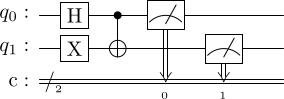
\includegraphics[width = .27 \linewidth]{images/Lab5_part3_circuit.png}
    \end{center}
    For reproducability the code that was used to simulate the quantum circuit is provided.
    \begin{verbatim}
        qc_mod = QuantumCircuit(2,2)
        qc_mod.x(1)
        qc_mod.h(0)
        qc_mod.cx(0,1)
        qc_mod.measure(0,0)
        qc_mod.measure(1,1)
        shots_mod = 1024
        job_mod = simulator.run([qc_mod], shots = shots_mod)
        plot_histogram(job_mod.result().get_counts(0))
    \end{verbatim}
    \subsection{Results}
    \begin{center}
        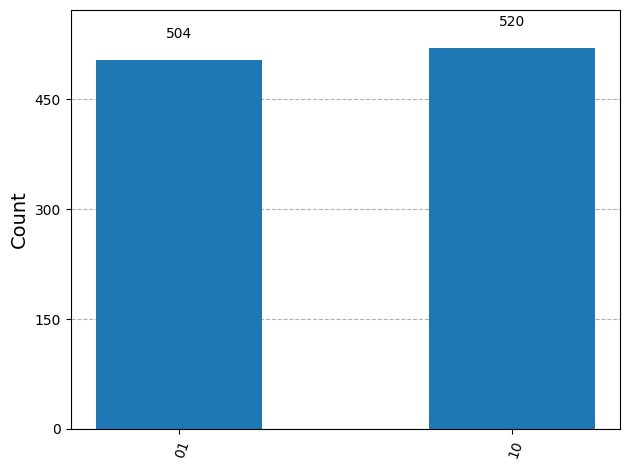
\includegraphics[width = .7 \linewidth]{images/Lab5_part3_hist.png}
    \end{center}
    The result of the simulation shows that the number of shots that were measured in the $\ket{01}$ state was 504 compared to the 520 shots measured in $\ket{10}$.
    The total number of shots ran was 1024, which means we had $\frac{504}{1024} \approx 49\%$ of the measurements result in $\ket{01}$ and $\frac{520}{1024} \approx 51\%$ of the measurements result in $\ket{10}$ which is within the 5\% error margin expected.
    These percentages add up to 100\%, which is expected as the only two results shown in the histogram are $\ket{01}$ and $\ket{10}$.
    \section{Design Challenge}
    \subsection{Calculations}
    Using the same basis states, we need to make a modified version of the Bell State where instead of a 50/50 split between $\ket{00}$ and $\ket{11}$ we have a 75/25 split.
    The Hadamard gate preforms a rotaton on the qubit gate 90 degress about the y-axis. So instead we can preform a rotation about the y-axis that gives us the wanted 75/25 split.
    So the fllowing circuit
    \begin{equation}
        RY_\theta\ket{0} = \alpha \ket{0} + \beta \ket{1}
    \end{equation}
    where we want ${\left|\alpha\right|}^2 = .75$ and ${\left|\beta\right|}^2 = .25$. Since we are rotating around the y-axs which is where we get imaginary values in the probablity ampltudes, $\alpha$ and $\beta$ should be real.
    From here we can say we want $\alpha = \sqrt{.75} = \frac{\sqrt{3}}{2}$ and $\beta = \sqrt{.25} = \frac{1}{2}$. Knowing that these are the values associated with the angle $\theta = \frac{\pi}{3} = 60^\circ$, we can say,
    \begin{equation}
        RY_\frac{\pi}{3}\ket{0} = \frac{\sqrt{3}}{2} \ket{0} + \frac{1}{2} \ket{1}.
    \end{equation}
    Which means
    \begin{equation*}
        \text{CNOT}\left(RY_\frac{\pi}{3}\otimes I\right) \ket{00} =
        \text{CNOT}\left(\frac{\sqrt{3}}{2} \ket{00} + \frac{1}{2} \ket{10} \right)=
        \frac{\sqrt{3}}{2} \ket{00} + \frac{1}{2} \ket{11}
    \end{equation*}
    \subsection{Code}
    The circuit to implement the modified bell states is shown below.
    \begin{center}
            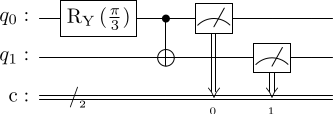
\includegraphics[width = .27 \linewidth]{images/Lab5_part4_circuit.png}
    \end{center}
    For reproducability the code that was used to simulate the quantum circuit is provided.
    \begin{verbatim}
        qc_design = QuantumCircuit(2,2)
        qc_design.ry(np.deg2rad(60),0)
        qc_design.cx(0,1)
        qc_design.measure(0,0)
        qc_design.measure(1,1)
        shots_design = 1024
        job_design = simulator.run([qc_design], shots = shots_design)
        plot_histogram(job_design.result().get_counts(0))
    \end{verbatim}
    \subsection{Results}
    \begin{center}
        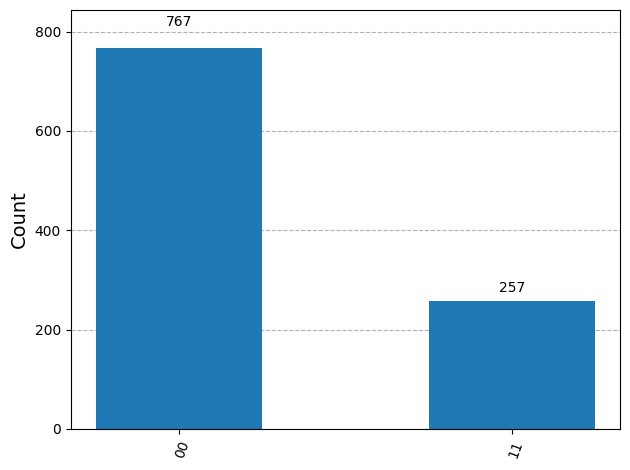
\includegraphics[width = .7 \linewidth]{images/Lab5_part4_hist.png}
    \end{center}
    The result of the simulation shows that the number of shots that were measured in the $\ket{00}$ state was 767 compared to the 257 shots measured in $\ket{10}$.
    The total number of shots ran was 1024, which means we had $\frac{767}{1024} \approx 74.9\%$ of the measurements result in $\ket{00}$ and $\frac{257}{1024} \approx 25.1\%$ of the measurements result in $\ket{11}$ which is within the 5\% error margin expected.
    These percentages add up to 100\%, which is expected as the only two results shown in the histogram are $\ket{00}$ and $\ket{11}$.
\end{document}